\section{Arrivée en Inde}

Date: 31/01/2008

\begin{multicols}{2}

Bonjour tout le monde,

Ca y est nous voila arrivés, le vol s'est très bien passé, et l'arrivée à l'aéroport était assez mouvementée... même à 1h du matin vous n'imaginez pas le monde qu'il peut y avoir dans l'aéroport de Delhi.

Premier passage obligé par arnaques et compagnie, il ne faut même pas faire confiance à la banque de l'Inde pour le change... résultat 400 roupies dans le vent (bon ok, pour nous c'est pas grand chose 1 euro = 56 roupies). Puis nous avons déjoué les arnaques du chauffeur de taxi qui nous emmène vers une office du tourisme à 2h du mat déjà c'est louche, alors quand on voit qu'il ne fait pas le bon numéro et qu'il a un petit sourire aux lèvres, plus confiance. Au final c'est nous qui avons guidé notre chauffeur qui faisait exprès de se perdre (et qui au final nous demande de repayer la course alors que c'était un taxi prépayé).

Au final nous voila dans un petit hôtel tout minable du vieux Delhi, en plein milieu de Main Bazar, mais qu'est-ce qu'on est heureux...

Petite précision : nous n'écrirons pas tous les jours comme ça, car à la vitesse d'internet ici ça prend beaucoup de temps.

A bientôt.

\hspace*{-0.65cm}
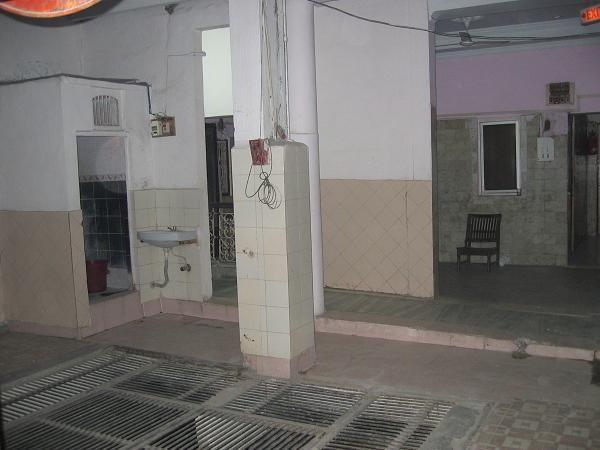
\includegraphics[width=4.8cm]{articles/Arrivee-en-inde/hotel.jpg}

Une petite photo de l'interieur de l'hôtel

\hspace*{-0.65cm}
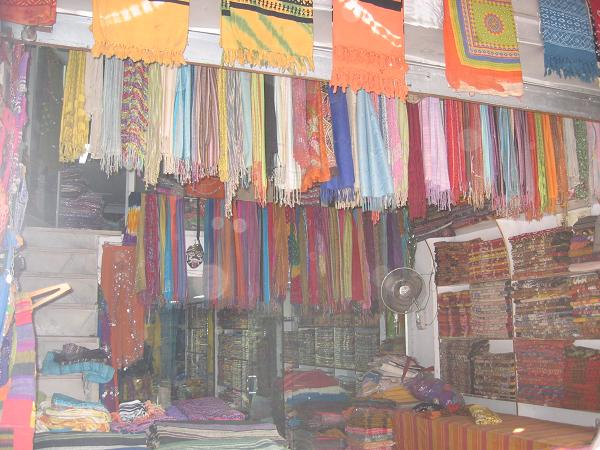
\includegraphics[width=4.8cm]{articles/Arrivee-en-inde/magasin.jpg}

Une boutique de main bazar

\hspace*{-0.65cm}
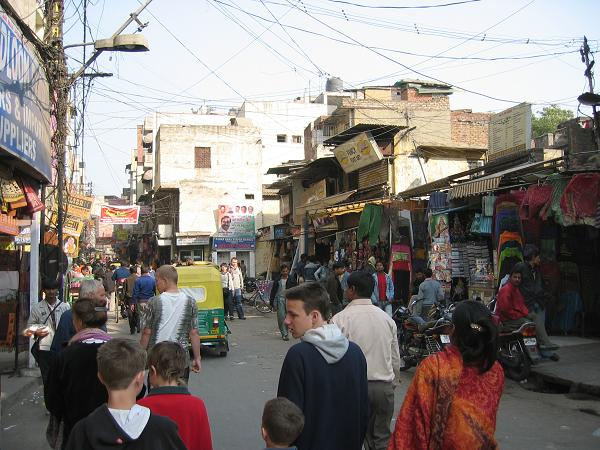
\includegraphics[width=4.8cm]{articles/Arrivee-en-inde/rue.jpg}
L'artère de main bazar, vue de devant l'hôtel

\end{multicols}
